\subsection{Tic Tac Toe}

\subsubsection{Backpropagation padrão}

O backpropagation padrão foi executado para a base de dados Tic Tac Toe com os seguintes parâmetros:

\begin{itemize}
	\item \texttt{size}: 5
	\item \texttt{learnFuncParams}: 0.1
	\item \texttt{maxit}: 50
\end{itemize}

A confusion matrix de uma execução é apresentada na Figura \ref{figura-confusion-matrix-tic-tac-toe-backpropagation-padrao}.

\begin{figure}[h!]
  \centering
  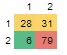
\includegraphics[width=0.3\linewidth]{figs/confusion-matrix-tic-tac-toe-backpropagation-padrao.png}
  \caption{Confusion Matrix - Tic Tac Toe - Backpropagation Padrão}
  \label{figura-confusion-matrix-tic-tac-toe-backpropagation-padrao}
\end{figure}

Os resultados para as 10 execuções do backpropagation padrão com as taxas de acertividade são apresentados na Tabela \ref{tabela-resultado-tic-tac-toe-backpropagation-padrao}. A média de acertividade foi de $0.7833$, com desvio padrão de $0.0401$.

\begin{table}[h!]
\centering
\caption{Resultados - Tic Tac Toe - Backpropagation padrão}
\label{tabela-resultado-tic-tac-toe-backpropagation-padrao}
\begin{tabular}{ll}
\toprule
                       & \textbf{Acertividade}       \\ \midrule
Execução 1             & 0.7500          \\
Execução 2             & 0.7986          \\
Execução 3             & 0.7500          \\
Execução 4             & 0.7778           \\
Execução 5             & 0.7500          \\
Execução 6             & 0.7500           \\
Execução 7             & 0.8194           \\
Execução 8             & 0.8403          \\
Execução 9             & 0.7500           \\
Execução 10            & 0.8472           \\
\textbf{Média}         & \textbf{0.7833} \\ \bottomrule
\textbf{Desvio Padrão} & \textbf{0.0401}
\end{tabular}
\end{table}

%O erro iterativo é apresentado na Figura \ref{figura-erro-iterativo-tic-tac-toe-backpropagation-padrao}.
%
%\begin{figure}
%  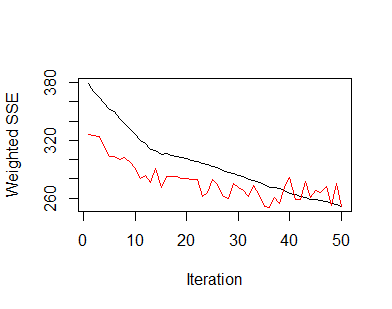
\includegraphics[width=\linewidth]{figs/erro-iterativo-tic-tac-toe-backpropagation-padrao.png}
%  \caption{Erro iterativo - Tic Tac Toe - Backpropagation Padrão}
%  \label{figura-erro-iterativo-tic-tac-toe-backpropagation-padrao}
%\end{figure}

\subsubsection{SCG}

O backpropagation com função de aprendizado SCG foi executado para a base de dados Tic Tac Toe com os seguintes parâmetros:

\begin{itemize}
	\item \texttt{size}: 5
	\item \texttt{learnFuncParams}: (0, 0, 0, 0)
	\item \texttt{maxit}: 50
\end{itemize}

A confusion matrix de uma execução é apresentada na Figura \ref{figura-confusion-matrix-tic-tac-toe-backpropagation-scg}.

\begin{figure}[h!]
  \centering
  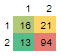
\includegraphics[width=0.3\linewidth]{figs/confusion-matrix-tic-tac-toe-backpropagation-scg.png}
  \caption{Confusion Matrix - Tic Tac Toe - Backpropagation SCG}
  \label{figura-confusion-matrix-tic-tac-toe-backpropagation-scg}
\end{figure}

Os resultados para as 10 execuções do backpropagation SCG com as taxas de acertividade são apresentados na Tabela \ref{tabela-resultado-wine-scg}. A média de acertividade foi de $0.7868$, com desvio padrão de $0.0656$.

\begin{table}[h!]
\centering
\caption{Resultados - Wine - Backpropagation SCG}
\label{tabela-resultado-wine-scg}
\begin{tabular}{ll}
\toprule
                       & \textbf{Acertividade}       \\ \midrule
Execução 1             & 0.7986          \\
Execução 2             & 0.7014          \\
Execução 3             & 0.9097           \\
Execução 4             & 0.7431          \\
Execução 5             & 0.6875           \\
Execução 6             & 0.8264          \\
Execução 7             & 0.8264           \\
Execução 8             & 0.7639           \\
Execução 9             & 0.8056          \\
Execução 10            & 0.8056          \\ \bottomrule
\textbf{Média}         & \textbf{0.7868} \\
\textbf{Desvio Padrão} & \textbf{0.0656}
\end{tabular}
\end{table}

%O erro iterativo é apresentado na Figura \ref{figura-erro-iterativo-tic-tac-toe-backpropagation-scg}.
%
%\begin{figure}
%  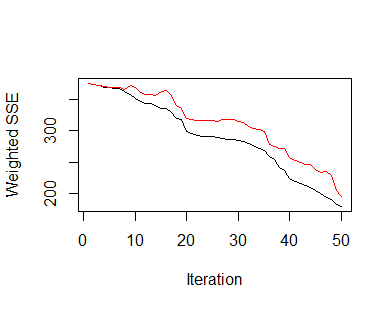
\includegraphics[width=\linewidth]{figs/erro-iterativo-tic-tac-toe-backpropagation-scg.png}
%  \caption{Erro iterativo - Tic Tac Toe - Backpropagation SCG}
%  \label{figura-erro-iterativo-tic-tac-toe-backpropagation-scg}
%\end{figure}